\mychapter{Metodologia}{cap:metod}\lhead{METODOLOGIA}

Este capítulo apresenta o arcabouço metodológico do AIPE, fundamentado na hipótese central de que o desempenho de políticas de reposição depende do regime operacional da demanda e que essa relação pode ser aprendida por um meta-modelo supervisionado. A metodologia organiza a camada de entrada (dados preparados, características operacionais e sinais auxiliares de previsão), o \textit{benchmark} das 12 políticas candidatas, a validação estatística, a geração de rótulos de política dominante e o treinamento do PSE. O primeiro experimento, conduzido como estudo piloto na Paraíba, validou o protocolo em escala controlada; o segundo experimento, conduzido com 145 séries da Bahia, ampliou o escopo empírico e incluiu validação estatística formal. A expansão nacional permanece como etapa futura de generalização.
\section{Visão Geral do AIPE}
\label{sec:visao_geral_aipe}

Nesta dissertação, o AIPE é a proposta metodológica principal: um \textit{framework} de seleção contextual de políticas de reposição. O PSE é seu componente de seleção, e as políticas avaliadas compõem o portfólio de alternativas sobre o qual o \textit{framework} aprende a recomendar.

Dados preparados, características das séries e sinais de previsão compõem a camada de entrada. O foco do AIPE está em transformar esses insumos em decisões de política por comparação empírica, validação estatística e aprendizado supervisionado; as etapas de entrada, tomadas isoladamente, não constituem a contribuição central.

Em seguida, as políticas candidatas são avaliadas em um ambiente de simulação comum. Para cada série, a política dominante é definida como aquela que apresenta o menor CTI entre as políticas operacionalmente viáveis, considerando o limiar mínimo de NS $\geq 0{,}70$. Quando nenhuma política satisfaz esse limiar, seleciona-se a alternativa de maior NS, conforme formalizado na Equação~\ref{eq:policy_selector}. Esses rótulos alimentam o PSE, cuja saída é uma recomendação de política de reposição para novas séries loja-produto.

O aprendizado de máquina aparece em dois níveis distintos na metodologia. No primeiro, métodos baseados em aprendizado por reforço, como DQN, PPO e SARSA, são políticas candidatas comparadas às políticas clássicas, às políticas parametrizadas por meta-heurísticas e às políticas híbridas. No segundo, o PSE atua como meta-modelo supervisionado que aprende a escolher qual política candidata tende a ser mais adequada para cada perfil operacional de demanda.

A organização deste capítulo acompanha a arquitetura conceitual da Figura~\ref{fig:aipe_architecture} em camadas. As seções seguintes descrevem, em ordem: a formulação do problema e a camada de entrada (dados, caracterização das séries e sinais auxiliares de previsão); o portfólio de políticas candidatas e o ambiente de simulação; os protocolos de validação temporal e estatística; a geração de rótulos e o treinamento do PSE; e, por fim, a camada de aplicação. As seções finais de artefatos e protocolo experimental complementam a arquitetura com requisitos de rastreabilidade e execução reprodutível.

A Figura~\ref{fig:aipe_architecture} ilustra essa arquitetura: a camada de entrada (dados, características e sinais de previsão) alimenta o núcleo de seleção contextual, onde são avaliadas as políticas candidatas, gerados os rótulos e treinado o PSE. Essa organização facilita a aplicação do \textit{framework} a outros contextos, desde que a camada de entrada seja adaptada.

\begin{figure}[p]
\centering
\resizebox{0.98\textwidth}{!}{%
\begin{tikzpicture}[
    >=Stealth,
    every node/.style={font=\scriptsize\sffamily},
    layer/.style={rectangle, draw=black!55, rounded corners=4pt, fill=gray!5, inner sep=7pt},
    title/.style={font=\bfseries\small\sffamily, align=center},
    box/.style={rectangle, draw=black!55, rounded corners=3pt, align=center, fill=white, text width=4.05cm, minimum height=1.35cm, inner sep=4pt},
    boxwide/.style={rectangle, draw=black!55, rounded corners=3pt, align=center, fill=white, text width=5.4cm, minimum height=1.35cm, inner sep=4pt},
    core/.style={rectangle, draw=black!65, rounded corners=3pt, align=center, fill=gray!10, text width=4.7cm, minimum height=1.25cm, inner sep=4pt},
    flow/.style={->, thick, black!70},
    feedback/.style={->, thick, dashed, black!60}
]

\node[title] (adaptTitle) at (0, 0) {Camada de entrada};
\node[box] (base) at (-2.9, -0.9) {
    \textbf{Base transacional}\\
    vendas; lojas; produtos;\\
    calendário/ciclos
};
\node[box] (params) at (2.9, -0.9) {
    \textbf{Parâmetros locais}\\
    custos; \textit{lead time};\\
    regras operacionais
};
\node[boxwide] (prep) at (0, -2.45) {
    \textbf{Padronização e preparação}\\
    série loja-produto; filtros;\\
    tratamento de zeros; agregação temporal
};
\node[box] (features) at (-2.9, -4.05) {
    \textbf{Características das séries}\\
    ADI; CV$^2$; volume;\\
    POD; sazonalidade
};
\node[box] (forecast) at (2.9, -4.05) {
    \textbf{Sinais auxiliares}\\
    métricas de previsão;\\
    sinais prospectivos
};
\begin{pgfonlayer}{background}
\node[layer, fit=(adaptTitle)(base)(params)(prep)(features)(forecast)] (adaptLayer) {};
\end{pgfonlayer}
\node[title] at (adaptTitle) {Camada de entrada};
\draw[flow, shorten >=2pt] (base.south) to[out=-90,in=130] ([xshift=-1.25cm]prep.north);
\draw[flow, shorten >=2pt] (params.south) to[out=-90,in=50] ([xshift=1.25cm]prep.north);
\draw[flow] (prep.south) to[out=-90,in=90] (features.north);
\draw[flow] (prep.south) to[out=-90,in=90] (forecast.north);

\node[title, below=1.05cm of forecast, xshift=-2.9cm] (coreTitle) {Núcleo de seleção contextual do AIPE};
\node[core, below=0.45cm of coreTitle, xshift=-3.0cm] (portfolio) {
    \textbf{Portfólio de políticas candidatas}\\
    clássicas: EOQ; $(s,S)$; Jornaleiro;\\
    parametrizadas: GA; SA; PSO; DE;\\
    RL: DQN; PPO; SARSA; híbridas GA-RL
};
\node[core, below=0.45cm of coreTitle, xshift=3.0cm] (sim) {
    \textbf{Ambiente de simulação}\\
    dinâmica de estoque; pedidos;\\
    \textit{lead time}; custos; falta de estoque
};
\node[core, below=0.50cm of portfolio, xshift=3.0cm] (eval) {
    \textbf{Avaliação comparativa}\\
    CTI; NS; TR; BE; FP
};
\node[core, below=0.50cm of sim, xshift=-3.0cm] (stats) {
    \textbf{Validação estatística}\\
    Wilcoxon; Friedman/Nemenyi;\\
    Cohen's $d$
};
\node[core, below=0.50cm of eval] (labels) {
    \textbf{Geração de rótulos}\\
    perfil operacional $\rightarrow$ política dominante;\\
    critérios de viabilidade operacional
};
\node[core, below=0.45cm of labels] (pse) {
    \textbf{\textit{Policy Selection Engine}: PSE}\\
    aprende a partir das entradas\\
    $\rightarrow$ política recomendada
};
\begin{pgfonlayer}{background}
\node[layer, fit=(coreTitle)(portfolio)(sim)(eval)(stats)(labels)(pse)] (coreLayer) {};
\end{pgfonlayer}
\node[title] at (coreTitle) {Núcleo de seleção contextual do AIPE};

\draw[flow] (features.south) to[out=-90,in=90] (portfolio.north);
\draw[flow] (forecast.south) to[out=-90,in=90] (sim.north);
\draw[flow] (features.south) to[out=-90,in=90] (sim.north);
\draw[flow] (portfolio) -- (eval);
\draw[flow] (sim) -- (stats);
\draw[flow] (eval) -- (labels);
\draw[flow] (stats) -- (labels);
\draw[flow] (labels) -- (pse);

\node[title, below=1.05cm of pse] (appTitle) {Camada de aplicação};
\node[box, below=0.35cm of appTitle, xshift=-5.2cm] (newseries) {
    \textbf{Nova série loja-produto}\\
    histórico recente;\\
    parâmetros operacionais
};
\node[box, below=0.35cm of appTitle] (recommendation) {
    \textbf{Recomendação do PSE}\\
    política recomendada; \textit{ranking};\\
    justificativa por perfil
};
\node[box, below=0.35cm of appTitle, xshift=5.2cm] (reeval) {
    \textbf{Reavaliação periódica}\\
    novos dados atualizam\\
    características, POD e recomendação
};
\begin{pgfonlayer}{background}
\node[layer, fit=(appTitle)(newseries)(recommendation)(reeval)] (appLayer) {};
\end{pgfonlayer}
\node[title] at (appTitle) {Camada de aplicação};

\draw[flow] (pse) -- (recommendation);
\draw[flow] (newseries) -- (recommendation);
\draw[flow] (recommendation) -- (reeval);
\coordinate (rightpath) at ([xshift=1.5cm]reeval.east);
\draw[feedback]
    (reeval.east)
    -- (reeval.east   -| rightpath)
    -- (forecast.east -| rightpath)
    -- (forecast.east)
    node[pos=0.38, right=4pt, align=center, font=\scriptsize\sffamily] {ciclo\\adaptativo};

\end{tikzpicture}}
\caption{Arquitetura conceitual do \textit{framework} AIPE. A camada de entrada reúne dados transacionais preparados, parâmetros operacionais, características das séries e sinais auxiliares de previsão de demanda. O núcleo de seleção contextual utiliza essas entradas para avaliar políticas candidatas, gerar rótulos de política dominante, realizar validação estatística e treinar o \textit{Policy Selection Engine}. A camada de aplicação utiliza o PSE para recomendar políticas a novas séries loja-produto e reavaliar periodicamente as recomendações conforme novos dados se acumulam.}
\label{fig:aipe_architecture}
\end{figure}


A leitura da Figura~\ref{fig:aipe_architecture} deve ser feita de cima para baixo. Na camada de entrada, a base transacional e os parâmetros locais são padronizados em séries loja-produto comparáveis; em seguida, extraem-se características operacionais, PODs e sinais auxiliares de previsão. No núcleo de seleção contextual, o portfólio reúne políticas clássicas, políticas parametrizadas por meta-heurísticas, políticas aprendidas por reforço e políticas híbridas GA-RL. Todas são executadas no mesmo ambiente de simulação, gerando os KPIs usados na avaliação comparativa, nos testes estatísticos e na construção dos rótulos de política dominante. O PSE aprende esses rótulos a partir das entradas operacionais. Na camada de aplicação, uma nova série é descrita pelo mesmo vetor de entrada, recebe uma recomendação ranqueada e pode ser reavaliada periodicamente conforme novos ciclos de venda alteram suas características.

\section{Instanciação Experimental do Problema de Inventário}
\label{sec:formulacao}

O Capítulo~\ref{cap:tec} apresentou a formulação conceitual do controle de inventário e as famílias de políticas de reposição. Nesta seção, essa formulação é instanciada para o \textit{benchmark} empírico: definem-se as decisões observadas em cada série loja-produto, a estrutura de rede, os parâmetros operacionais locais e a forma como as métricas são calculadas sob condições comparáveis.

\subsection{Instanciação das Políticas e Espaço de Decisão}

A definição formal de política de reposição foi apresentada no Capítulo~\ref{cap:tec}. Na metodologia, essa definição é operacionalizada para cada série loja-produto: no ciclo $t$, a política recebe o estado observado da loja $i$ e retorna uma quantidade de pedido não negativa:
\[
  Q_{t,i} = \pi(I_{t,i},\, D_{t-1,i},\, Q_{t-L,i};\, \boldsymbol{\theta}),
\]
em que $I_{t,i}$ representa o estoque disponível, $D_{t-1,i}$ resume a demanda recente, $Q_{t-L,i}$ indica pedidos em trânsito recebidos após o prazo de entrega e $\boldsymbol{\theta}$ é o vetor de parâmetros da política. Esse vetor assume naturezas distintas conforme a família candidata, como pares $(s,Q)$ em políticas parametrizadas ou pesos de rede neural em agentes de aprendizado por reforço.

Esta distinção é essencial: as 12 políticas avaliadas são instâncias de famílias distintas; o AIPE é a estratégia adaptativa que aprende qual família e parâmetros usar por série. Assim, o foco metodológico está na seleção contextual, e não na defesa de uma política isolada como solução universal.

\begin{defi}[Seleção Adaptativa de Política (AIPE)]
Dado o espaço de séries $\mathcal{X}$, o mapeamento de características $\phi: \mathcal{X} \rightarrow \mathbb{R}^p$ e o conjunto de políticas candidatas $\Pi = \{\pi_1, \ldots, \pi_k\}$, o \textit{Policy Selection Engine} aprende a função:
\[
  f: \mathbb{R}^p \rightarrow \Pi, \qquad f\!\bigl(\phi(\mathbf{x}_i)\bigr) = \hat{\pi}^*(i),
\]
tal que $\hat{\pi}^*(i) \approx \arg\min_{\pi \in \Pi} \mathbb{E}[\mathrm{CTI}(\pi, \mathbf{x}_i)]$ sujeito a $\mathbb{E}[\mathrm{NS}(\pi, \mathbf{x}_i)] \geq \alpha_{\min}$. O \textit{Adaptive Inventory Policy Engine} (AIPE) implementa $f$ como meta-modelo supervisionado treinado sobre os pares $\{(\phi(\mathbf{x}_i),\, \hat{\pi}^*(i))\}_{i=1}^N$ gerados pelo \textit{benchmark}, com reavaliação periódica de $\phi(\mathbf{x}_i)$ a cada $\Delta t$ ciclos.
\end{defi}

\subsection{Instanciação do Ambiente de Inventário}

O ambiente experimental especializa o modelo do Capítulo~\ref{cap:tec} para uma rede com $N$ lojas varejistas atendidas por um armazém central. O horizonte de planejamento é discretizado em ciclos comerciais $t \in \{1, \ldots, T\}$, cada um com aproximadamente 21 dias corridos. As variáveis e parâmetros usados na simulação são:

\begin{itemize}
  \item $D_{t,i} \geq 0$: demanda observada na loja $i$ no ciclo $t$;
  \item $I_{t,i}$: nível de estoque da loja $i$ no início de $t$;
  \item $Q_{t,i} \geq 0$: quantidade pedida em $t$, recebida após prazo $L$ ciclos;
  \item $S_{t,i} = \max(0, D_{t,i} - I_{t,i})$: ruptura no ciclo $t$;
  \item $h$, $c_s$, $c_o^{\text{fix}}$, $c_o^{\text{var}}$: custos unitários de manutenção, ruptura, ordenação fixa e variável.
\end{itemize}

O custo acumulado usado no \textit{benchmark} corresponde à versão operacional, indexada por loja, da Equação~\ref{eq:obj_inv_control}. Para cada política candidata, calcula-se:

\begin{equation}
  \min_\pi \sum_{t=1}^{T} \bigl[
    h\, I_{t,i} + c_s\, S_{t,i}
    + c_o^{\text{fix}}\,\mathbf{1}(Q_{t,i}>0)
    + c_o^{\text{var}}\, Q_{t,i}
  \bigr],
  \label{eq:obj_meio}
\end{equation}

Na Equação~\ref{eq:obj_meio}, a função indicadora $\mathbf{1}(Q_{t,i}>0)$ assume valor 1 quando há emissão de pedido no ciclo $t$ e 0 caso contrário. O cálculo é repetido para cada série loja-produto e depois agregado por política, permitindo comparar alternativas sob o mesmo ambiente de avaliação.

A dinâmica simulada é a versão indexada por loja da Equação~\ref{eq:balance}:

\begin{equation}
  I_{t+1,i} = \max\bigl(0,\; I_{t,i} - D_{t,i}\bigr) + Q_{t-L,i}, \quad \forall\, t,\; \forall\, i.
  \label{eq:balance_meio}
\end{equation}

Na Equação~\ref{eq:balance_meio}, o operador $\max(0,\cdot)$ representa o pressuposto de venda perdida: a demanda que excede o estoque disponível não é acumulada para ciclos futuros. O termo $Q_{t-L,i}$ representa pedidos emitidos $L$ ciclos antes e recebidos no ciclo corrente.

\subsection{Rede Varejista}

A cadeia de suprimentos modela três escalões hierárquicos:

\begin{itemize}
  \item Escalão 1 (Armazém Regional): único centro distribuidor; repõe junto ao fornecedor com prazo $L$ ciclos.
  \item Escalão 2 (Lojas Revendedoras): $N$ unidades varejistas com séries de demanda independentes; cada loja decide individualmente quando e quanto pedir ao armazém (política descentralizada).
  \item Escalão 3 (Produto): conjunto de produtos do portfólio da rede. No primeiro experimento, um único produto de alta intermitência foi usado para controle experimental; no segundo experimento, o recorte foi ampliado para múltiplos produtos ativos com filtragem por regime de demanda (Syntetos-Boylan).
\end{itemize}

\subsection{Métricas de Avaliação}
\label{sec:metricas_avaliacao}

As métricas já foram definidas conceitualmente no Capítulo~\ref{cap:tec}; aqui elas são retomadas apenas para explicitar como o \textit{benchmark} calcula o desempenho de cada política em cada série. Ao fim de $T$ ciclos, cinco indicadores são registrados para cada combinação (política, loja):

\begin{itemize}
  \item \textit{CTI} (Custo Total de Inventário): $\sum_{t}[h I_t + c_s S_t + c_o^{\text{fix}}\mathbf{1}(Q_t>0) + c_o^{\text{var}}Q_t]$;
  \item \textit{NS} (Nível de Serviço): $\sum_t \min(I_t, D_t) / \sum_t D_t$;
  \item \textit{TR} (Taxa de Ruptura): frequência de ciclos com falta de estoque (\textit{stockout}); ao longo do texto, ``ruptura'' é empregado como equivalente técnico de ``falta de estoque'';
  \item \textit{BE} (\textit{Bullwhip Effect}): $\mathrm{Var}(Q)/\mathrm{Var}(D)$, amplificação da variabilidade ao longo da cadeia;
  \item \textit{FP} (Frequência de Pedidos): fração de ciclos com ao menos um pedido emitido.
\end{itemize}

Esses cinco indicadores formam a base comparativa das políticas candidatas. No segundo experimento, eles são complementados por métricas de previsão (MASE, sMAPE, RMSSE) usadas como sinais auxiliares para o PSE. Assim, a metodologia não escolhe o melhor modelo de previsão como fim em si mesmo; ela avalia se esses sinais aumentam a capacidade de selecionar políticas de reposição de forma contextual.

Além do CTI original, usado como custo direto de inventário, esta dissertação reporta uma métrica complementar de custo operacional ajustado por estabilidade. Essa métrica combina o CTI normalizado e uma penalidade baseada no BE normalizado, permitindo avaliar se políticas de menor custo direto também preservam estabilidade nos pedidos enviados ao armazém:
\begin{equation}
J(\pi, g) = \mathrm{CTI}_{\text{norm}}(\pi, g) + \lambda_{BE} \cdot \mathrm{BE}_{\text{norm}}(\pi, g)
\end{equation}
em que $\pi$ é a política, $g$ é o perfil operacional (ou o conjunto global, no caso da política única), $\mathrm{CTI}_{\text{norm}}$ e $\mathrm{BE}_{\text{norm}}$ são o CTI e o BE normalizados por min-max sobre o conjunto de políticas avaliadas, e $\lambda_{BE} \geq 0$ é o peso da penalidade por instabilidade: $\lambda_{BE}=0$ recupera o custo puro (equivalente a ordenar apenas por CTI); valores de $\lambda_{BE} > 0$ aumentam a penalização de políticas com efeito \textit{bullwhip} elevado. O CTI ajustado não substitui o CTI original; ele é reportado como análise complementar de sensibilidade (Seção~\ref{sec:custo_politica_unica_vs_perfil}), de caráter preliminar, para apoiar a discussão sobre seleção contextual de políticas considerando custo e estabilidade conjuntamente.

\section{Camada de Entrada: Dados e Pré-Processamento}

Esta seção descreve o conjunto de dados transacional utilizado nos experimentos e os estágios de pré-processamento que transformam os registros brutos em séries prontas para simulação. A descrição também explicita as escolhas de filtragem que delimitam o escopo empírico do estudo piloto e da expansão experimental.

\subsection{Base de Dados}

Os dados provêm de uma base transacional de gestão de vendas de uma rede de varejo do Nordeste brasileiro. O conjunto completo compreende aproximadamente 48 milhões de transações, cobrindo 26 estados e o DF, com cerca de 12 mil produtos e 3 milhões de pares (loja, produto) ao longo de 38 ciclos comerciais (janeiro/2023 a abril/2025). O \textit{dataset} é proprietário e de acesso restrito. A rastreabilidade do \textit{pipeline} permite reproduzir integralmente todos os experimentos a partir dos dados originais, configurações e código-fonte com sementes aleatórias fixas.

A Tabela~\ref{tab:dataset_stats} resume as principais características do \textit{dataset} nos dois experimentos executados. Essa síntese é usada apenas para delimitar o escopo metodológico; a análise empírica detalhada de distribuição geográfica, perfis e desempenho das políticas é apresentada no Capítulo~\ref{cap:results}.

\begin{table}[ht]
\centering
\small
\caption{Características do \textit{dataset} por experimento.}
\label{tab:dataset_stats}
\begin{tabular}{@{}lcc@{}}
\toprule
Característica & Experimento 1 (PB) & Experimento 2 (BA) \\
\midrule
Estados cobertos                      & 1 (PB)    & 1 (BA) \\
Lojas ativas                          & 15        & $\sim$40 \\
Produtos avaliados                   & 1 (48130) & $\sim$10 \\
Séries (loja, produto) após filtragem     & 15        & 145 \\
Ciclos por série ($T$)                & 38        & 38 \\
Ciclos com demanda positiva (mediana) & 19        & 17 \\
ADI médio (intermitência)             & 2.1       & 2.4 \\
CV$^2$ médio (irregularidade)         & 3.8       & 4.1 \\
\% séries no quadrante \textit{Lumpy} & 67\%      & 71\% \\
Replicações independentes             & 1         & 5 \\
Pontos de avaliação totais            & 180       & 8.700 \\
\bottomrule
\end{tabular}
\end{table}

A dominância do quadrante \textit{Lumpy} (ADI $>1.32$ e CV$^2 > 0.49$) nos dois experimentos delimita um contexto de demanda intermitente e irregular: vendas concentradas em poucas revendedoras ativas por ciclo, com picos de grande magnitude. Esse regime é desafiador para políticas clássicas e justifica a avaliação de seleção contextual, sem pressupor que uma única política seja superior em todas as séries.

O primeiro experimento aplica um recorte controlado: estado da Paraíba, produto único (48130, alta intermitência), lojas com $\geq 17$ ciclos com demanda positiva. Esse recorte foi usado para validar a dinâmica experimental em escala reduzida antes da ampliação do portfólio.

O segundo experimento expande o escopo para o estado da Bahia e para múltiplos produtos ativos. A filtragem automática seleciona séries com CV $\geq 1.5$ e ciclos positivos suficientes para discriminar entre políticas. A extensão para todos os estados brasileiros compõe a etapa futura de generalização nacional.

\subsection{Estrutura Temporal}

A base registra vendas por \textit{ciclo comercial} (17 ciclos por ano, $\approx$21 dias corridos cada). Essa granularidade reflete a política operacional real: pedidos são consolidados e processados por ciclo, justificando o prazo $L=2$ ciclos ($\approx$42 dias). Com essa granularidade, um horizonte de 38 ciclos (janeiro/2023 a abril/2025) captura: (i) sazonalidade anual completa (variações de demanda por mês/período), (ii) múltiplos padrões de intermitência (ciclos com venda zero e picos concentrados), e (iii) estabilização de parâmetros de estimação, crucial para validação confiável.

\subsection{Regimes de Demanda}

Após a agregação por ciclo, cada série (loja, produto) é caracterizada pelos índices de Syntetos-Boylan (Seção~\ref{sec:sb_taxa}) e classificada em um dos quatro quadrantes: \textit{Smooth} (ADI $\leq 1.32$, CV$^2 \leq 0.49$), \textit{Erratic} (ADI $\leq 1.32$, CV$^2 > 0.49$), \textit{Intermittent} (ADI $> 1.32$, CV$^2 \leq 0.49$) e \textit{Lumpy} (ADI $> 1.32$, CV$^2 > 0.49$). A Figura~\ref{fig:aipe_decision_flow} integra essa classificação ao fluxo decisório geral do AIPE.

A heterogeneidade dos regimes no \textit{dataset} é marcante: o ADI varia de $1.02$ a $8.7$ e o CV$^2$ de $0.8$ a $18.4$ nas séries do segundo experimento, cobrindo desde séries quase regulares até padrões de demanda extremamente esporádica. Essa diversidade é um ativo central do estudo: a superioridade de uma política em relação a outra varia sistematicamente com a posição da série no plano ADI $\times$ CV$^2$, e é exatamente essa relação que o PSE aprende a partir das entradas operacionais. Essa classificação orienta a estratificação das análises e a seleção de modelos de previsão e políticas recomendadas por regime.

\subsection{Pipeline Experimental}

O pré-processamento transforma dados transacionais brutos em séries de demanda estruturadas para simulação. Esse \textit{pipeline} é essencial porque: (i) dados brutos contêm inconsistências, (ii) a granularidade deve refletir decisões operacionais reais, (iii) séries devem ter qualidade suficiente para discriminar entre políticas. As etapas são:

\begin{enumerate}[(i)]
  \item Filtragem: exclusão de registros com revendedora inativa, remoção de transações anômalas (tipo brinde, quantidades negativas) e restrição ao período de análise (janeiro/2023 a abril/2025);

  \item Limpeza: imputação de ciclos ausentes com demanda zero, garantindo série de comprimento uniforme $T=38$;

  \item Agregação: soma de quantidades por (loja, produto, ciclo comercial), transformando registros transacionais em séries de demanda agregadas;

  \item Seleção de cenários: filtragem automática por critérios de qualidade (coeficiente de variação $\geq 1.5$ para capturar intermitência, mínimo de ciclos com demanda positiva, produto ativo nos últimos 3 ciclos), produzindo o conjunto de séries para análise.
\end{enumerate}

Essa sequência elimina inconsistências e produz um conjunto de séries (loja, produto) prontas para engenharia de características e simulação. Com isso, as etapas posteriores operam sobre séries uniformes e comparáveis.

\section{Caracterização das Séries e Perfis Operacionais}
\label{sec:carac_series}

As características operacionais da demanda compõem a representação de entrada utilizada pelo AIPE. A taxonomia de Syntetos-Boylan fornece uma caracterização inicial baseada na frequência de ocorrência de demanda positiva (ADI) e na variabilidade relativa da magnitude da demanda (CV$^2$), enquanto as demais características ampliam essa representação com informações de volume, sazonalidade, concentração de picos, dispersão e estabilidade temporal. Em conjunto, essas variáveis descrevem o perfil operacional de cada série e permitem que o PSE aprenda associações entre padrões de demanda e políticas de reposição com melhor desempenho esperado.

O estágio \texttt{demand\_profiling} (nome do módulo computacional) estende a classificação Syntetos-Boylan, produzindo um vetor de 17 características operacionais por série e agrupando as séries em perfis orientados à decisão de política. Esse vetor permanece como insumo para o mecanismo de seleção contextual, não como uma recomendação final por si só.

\subsection{Objetivo da Caracterização}

A classificação Syntetos-Boylan (Seção~\ref{sec:sb_taxa}) usa apenas dois índices (ADI e CV$^2$) e identifica o regime de cada série. Para o \textit{Policy Selection Engine} (Seção seguinte), é necessário um vetor de características mais rico, que capture não apenas a intermitência, mas também a estrutura temporal, a distribuição e o comportamento operacional de cada série. O estágio \texttt{demand\_profiling} produz esse vetor.

\subsection{Características Operacionais Calculadas}

Para cada série $(w, s, i)$, em que $w$ identifica a loja, $s$ identifica o produto e $i$ indexa a série loja-produto no conjunto experimental, calculam-se 17 características numéricas organizadas em quatro grupos:

\paragraph{Características de intermitência:}
\begin{itemize}
  \item $\text{ADI} = T / n^+$: intervalo médio entre demandas positivas (Average Demand Interval);
  \item $\text{CV}^2 = (\sigma/\mu)^2$: variabilidade normalizada das quantidades;
  \item $r_0 = 1 - n^+/T$: proporção de ciclos com demanda zero, em que $n^+$ é o número de ciclos com demanda positiva;
  \item $z_{\max}$, $z_{\text{mean}}$: comprimento máximo e médio das sequências de zeros consecutivos;
  \item $B = (s_\tau - \bar{\tau}) / (s_\tau + \bar{\tau})$: \textit{burstiness}~\citep{GohBarabasi2008Burstiness}, onde $\tau_i$ são os intervalos entre eventos de demanda, $\bar{\tau}$ é a média desses intervalos e $s_\tau$ é seu desvio-padrão; $B \in [-1, 1]$, com $B > 0$ indicando clusters de demanda e $B < 0$ indicando demanda regular.
\end{itemize}

\paragraph{Características de distribuição (sobre valores positivos):}
\begin{itemize}
  \item \textit{Assimetria} e \textit{curtose excedente} dos tamanhos de demanda positivos;
  \item \textit{Entropia de Shannon}: $H = -\sum_k p_k \log_2 p_k$, calculada sobre histograma de 10 bins, em que $p_k$ é a proporção de observações no bin $k$; mede a difusividade da distribuição de demanda.
\end{itemize}

\paragraph{Características de tendência e sazonalidade:}
\begin{itemize}
  \item $\beta_t / \mu$: coeficiente angular OLS normalizado, em que $\beta_t$ é a inclinação estimada da série ao longo do tempo e $\mu$ é a média da demanda;
  \item $\rho_S$: autocorrelação da série no lag sazonal $S = 17$, em que $S$ representa um ano comercial completo.
\end{itemize}

\paragraph{Características de volume (herdadas de \texttt{scenarios\_meta}):}
$\mu$, $\sigma$, $n_T$, $n^+$, e as métricas de perfil da revendedora (segmento, filial, estrutura), em que $n_T$ representa o número total de ciclos observados. Esse grupo complementa as características de intermitência, variabilidade e sazonalidade com sinais de escala operacional.

\subsection{Perfis Operacionais de Demanda}

Com base nas características acima, cada série é classificada em um dos cinco \textit{Perfis Operacionais de Demanda} (POD) por regras hierárquicas (Tabela~\ref{tab:pod}). O POD é uma heurística operacional baseada em limiares interpretáveis, não um agrupamento obtido por algoritmo de \textit{clustering}. Ao contrário da classificação Syntetos-Boylan, o POD é orientado à decisão: seu objetivo é fornecer uma linguagem intermediária para o PSE, não apenas descrever o padrão de demanda. Na tabela, a coluna ``POD'' nomeia o perfil; ``Característica principal'' resume o comportamento dominante da demanda naquele perfil; ``Critério'' apresenta a regra hierárquica utilizada para classificar a série; e ``Política de referência inicial'' indica a associação usada pelo módulo de perfilamento antes do \textit{benchmark}. Essa associação não substitui a seleção final: a política dominante efetiva é definida posteriormente pela simulação, pela validação estatística e pelo critério da Equação~\ref{eq:policy_selector}.

\begin{table}[htbp]
\centering
\small
\caption{Perfis Operacionais de Demanda (POD) e políticas de referência inicial.}
\label{tab:pod}
\resizebox{\linewidth}{!}{%
\begin{tabular}{p{2.8cm}p{3.2cm}p{5.0cm}p{2.6cm}}
\toprule
POD & Característica principal & Critério & Política de referência inicial \\
\midrule
Sparse High Impact & Longos silêncios + picos & ADI $\geq 1.32$ e CV$^2 \geq 0.49$ e $z_{\max} \geq 5$ & GA-DQN \\
High Vol. Seasonal & Sazonalidade ou burstiness & $\rho_S \geq 0.25$ ou $B \geq 0.30$ & PPO \\
Unstable Trend     & Tendência ou distribuição difusa & $|\beta_t/\mu| \geq 0.05$ ou $H \geq 2.0$ & GA-PPO \\
Low Vol. Stable    & Baixo volume, baixa variação & $\mu \leq 2.0$ e CV$^2 < 0.49$ & Newsvendor \\
Fast Moving        & Demanda frequente & ADI $< 1.32$ & $(s,S)$ \\
\bottomrule
\end{tabular}
}% end resizebox
\end{table}

As regras são aplicadas de forma hierárquica, na ordem apresentada na Tabela~\ref{tab:pod}: primeiro são identificadas séries esparsas de alto impacto, depois padrões sazonais ou explosivos, séries com tendência ou distribuição difusa, séries estáveis de baixo volume e, por fim, séries de demanda frequente. Os limiares são configuráveis via \texttt{demand\_profiling.yml} e calibráveis por análise exploratória do \textit{dataset}. Essa parametrização preserva a reprodutibilidade e permite adaptar o perfilamento a outros recortes de dados.

O POD é a linguagem operacional usada como entrada pelo PSE: toda recomendação de política parte do perfil da série, não de características isoladas. O fluxo decisório completo organiza-se sequencialmente como:
\[
  \underbrace{\mathbf{x}_i}_{\text{série}} \;\xrightarrow{\;\phi\;}\; \underbrace{\phi(\mathbf{x}_i) \in \mathbb{R}^{17}}_{\text{características}} \;\xrightarrow{\;\mathrm{POD}\;}\; \underbrace{p \in \{1,\ldots,5\}}_{\text{perfil}} \;\xrightarrow{\;f\;}\; \underbrace{\hat{\pi}^*(i) \in \Pi}_{\text{política}} \;\xrightarrow{\;\mathrm{sim}\;}\; \underbrace{(\mathrm{CTI},\,\mathrm{NS},\,\mathrm{TR},\,\mathrm{BE},\,\mathrm{FP})}_{\text{KPIs esperados}}
\]
A generalização para séries não vistas é avaliada por validação cruzada estratificada.

\begin{figure}[ht]
\centering
\resizebox{\textwidth}{!}{%
\begin{tikzpicture}[
    >=Stealth,
    node distance=0.6cm and 0.5cm,
    box/.style={rectangle, draw, rounded corners=3pt, align=center,
                minimum width=2.2cm, minimum height=0.9cm, font=\small\sffamily,
                fill=gray!8},
    feedback/.style={->, thick, dashed, gray},
    flow/.style={->, thick}
]

\node[box]                       (hist)   {Histórico\\de Vendas};
\node[box, right=of hist]        (feat)   {Features\\$\phi(x_i) \in \mathbb{R}^{17}$};
\node[box, right=of feat]        (pod)    {POD\\$p \in \{1,\ldots,5\}$};
\node[box, right=of pod]         (pse)    {Policy\\Selection\\$f(\phi) \to \hat\pi^*$};
\node[box, right=of pse]         (sim)    {Simulação\\12 políticas};
\node[box, right=of sim]         (kpi)    {KPI\\(CTI, NS, BE)};
\node[box, below=0.9cm of pse, xshift=1.2cm]
                                  (reav)   {Reavaliação\\$\Delta t = 6$ ciclos};

\draw[flow] (hist) -- (feat);
\draw[flow] (feat) -- (pod);
\draw[flow] (pod)  -- (pse);
\draw[flow] (pse)  -- (sim);
\draw[flow] (sim)  -- (kpi);

\draw[feedback] (kpi.south) .. controls +(0,-0.85) and +(1.10,0.15) ..
  node[right, pos=0.55, font=\scriptsize\sffamily, align=center] {monitora\\desvio} (reav.east);
\draw[feedback] (reav.west) .. controls +(-0.95,0.30) and +(0,-0.85) ..
  node[left, pos=0.45, font=\scriptsize\sffamily, align=center] {atualiza\\características} (pod.south);

\end{tikzpicture}
}
\caption{Fluxo decisório do AIPE. O histórico preparado, as características operacionais e o POD formam a entrada usada pelo PSE para recomendar uma política; o ciclo de reavaliação periódica a cada $\Delta t=6$ ciclos (tracejado) recalcula as características e o POD conforme novos dados se acumulam, sem re-treinar o meta-modelo.}
\label{fig:aipe_decision_flow}
\end{figure}

\section{Sinais Auxiliares de Previsão de Demanda}
\label{sec:sinais_previsao}

A previsão de demanda fornece sinais auxiliares sobre o comportamento esperado de cada série, incorporados à camada de entrada e ao treinamento do PSE. Quatro modelos (Croston, ARIMA/SARIMAX, XGBoost e LSTM) são treinados por série e selecionados por validação \textit{walk-forward} com métrica MASE \citep{Croston1972ForecastingIntermittentDemand}. A janela mínima de treinamento é $T_{\min} = 12$ ciclos; cada passo avança um ciclo, produzindo 20 a 26 pontos de teste. O protocolo elimina viés \textit{in-sample} e garante que previsões respeitem a ordem temporal dos dados. O modelo com menor MASE é selecionado como \textit{forecaster} oficial da série e suas métricas de acurácia (MASE, sMAPE, RMSSE) são incorporadas como sinais auxiliares de entrada.

Os parâmetros de referência para as políticas ($I_0$, $Q_{\text{ref}}$, $s_{\text{ref}}$) são calculados a partir das estatísticas locais $\hat{\mu}$ e $\hat{\sigma}$ de cada série por calibração adaptativa:

\begin{align}
  I_0 &= \max\!\bigl(100,\; 2\hat{\mu} L\bigr), \label{eq:I0_metod}\\
  Q_{\text{ref}} &= \sqrt{2\hat{\mu} T\, c_o^{\text{fix}} / h}, \label{eq:qref_metod}\\
  s_{\text{ref}} &= \hat{\mu} L + z\hat{\sigma}\sqrt{L}, \label{eq:sref_metod}
\end{align}

com $z = 1.28$ (nível de serviço alvo de 90\%). Os espaços de busca das meta-heurísticas e os limites de ação dos agentes de RL são dimensionados proporcionalmente a $Q_{\text{ref}}$ e $s_{\text{ref}}$, garantindo comparação justa entre lojas com volumes heterogêneos (razão de até 124 vezes entre a maior e a menor loja no estudo piloto). No segundo experimento, $\hat{\mu}$ e $\hat{\sigma}$ são atualizados a cada ciclo com a janela deslizante, implementando calibração \textit{online}.
Nas Equações~\ref{eq:I0_metod} a~\ref{eq:sref_metod}, $I_0$ é o estoque inicial usado na simulação, $Q_{\text{ref}}$ é o lote de referência usado para dimensionar ações e limites de busca, $s_{\text{ref}}$ é o ponto de reposição de referência, $\hat{\mu}$ e $\hat{\sigma}$ são a média e o desvio-padrão estimados na janela histórica disponível, $T$ é o horizonte experimental, $L$ é o prazo de entrega, $c_o^{\text{fix}}$ é o custo fixo por pedido e $h$ é o custo de manutenção.

\section{Portfólio de Políticas Candidatas}
\label{sec:benchmark_massivo}

Esta seção descreve o portfólio de doze políticas candidatas organizadas em quatro famílias: políticas clássicas, políticas parametrizadas por meta-heurísticas, políticas aprendidas por reforço e políticas híbridas GA-RL. Nesta dissertação, ``política'' designa a regra que transforma um estado de inventário em uma decisão de reposição; GA, SA, PSO e DE são métodos de busca usados para parametrizar essa regra, não políticas autônomas no sentido decisório. Todas as alternativas são avaliadas no mesmo ambiente \textit{InventoryEnv} com as mesmas séries de demanda real, garantindo comparação controlada.

\subsection{Políticas Clássicas}

As políticas clássicas são regras analíticas ou semianalíticas de reposição. Elas definem diretamente quando pedir e quanto pedir a partir de parâmetros estimados da série, como demanda média, variabilidade e prazo de entrega. As representações visuais complementares dessas políticas, incluindo a política $(s,S)$, foram deslocadas para o Apêndice~\ref{ap:representacoes_politicas}, preservando no corpo do capítulo apenas sua formulação operacional.

\textit{EOQ.} $Q^* = \sqrt{2 D c_o^{\text{fix}} / h}$, em que $D$ é a demanda agregada estimada para o horizonte de referência, $c_o^{\text{fix}}$ é o custo fixo de pedido e $h$ é o custo de manutenção. O ponto de reposição é $s = \hat{\mu} L$. Pressupõe demanda constante, violada em regime intermitente.

\textit{$(s,S)$.} Pedido de magnitude $S - I_t$ sempre que $I_t \leq s$, em que $I_t$ é a posição de estoque no ciclo $t$, $s = s_{\text{EOQ}}$ é o ponto de disparo e $S = s + Q_{\text{EOQ}}$ é o nível-alvo. Política de referência amplamente usada no varejo regional brasileiro.

\textit{Jornaleiro.} $Q^* = \hat{\mu} + z\hat{\sigma}$, com $z = 1.28$, em que $\hat{\mu}$ e $\hat{\sigma}$ são a média e o desvio-padrão estimados da demanda. Determina o pedido ótimo de período único como quantil da distribuição de demanda. Representações visuais complementares do EOQ e do Jornaleiro são apresentadas no Apêndice~\ref{ap:representacoes_politicas}.

\subsection{Políticas Parametrizadas por Meta-Heurísticas}

Nas políticas parametrizadas por meta-heurísticas, cada solução candidata representa uma parametrização de uma regra de reposição por ponto de pedido. No recorte implementado, a solução é descrita por $\boldsymbol{\theta}=(s,Q)$, em que $s$ é o ponto de reposição e $Q$ é a quantidade de pedido. A política resultante emite um pedido de tamanho $Q$ quando a posição de estoque atinge o limiar $s$, respeitando os limites operacionais definidos para a série.

A função objetivo é definida antes da aplicação dos algoritmos de busca. Para uma série $i$, a meta-heurística procura:

\begin{equation}
  \boldsymbol{\theta}_i^*
  = \arg\min_{\boldsymbol{\theta} \in \Theta_i}
  \mathrm{CTI}(\pi_{\boldsymbol{\theta}}, i)
  \quad \text{sujeito a } \mathrm{NS}(\pi_{\boldsymbol{\theta}}, i) \geq \alpha_{\min},
  \label{eq:obj_metaheuristicas}
\end{equation}

\noindent em que $\Theta_i$ é o espaço viável de parâmetros da série $i$, $\pi_{\boldsymbol{\theta}}$ é a política induzida pelo par $(s,Q)$, CTI é calculado pela Equação~\ref{eq:obj_meio} e $\alpha_{\min}=0{,}70$ é o nível mínimo de serviço adotado na seleção contextual. Quando o algoritmo requer uma função escalar de aptidão, a restrição de serviço é implementada por penalização de candidatos inviáveis ou por descarte no momento de geração do rótulo. Assim, GA, SA, PSO e DE diferem no mecanismo de busca, mas compartilham a mesma representação, o mesmo ambiente de avaliação e os mesmos critérios de viabilidade operacional.

\textit{GA.} O Algoritmo Genético mantém uma população de parametrizações candidatas. Cada indivíduo codifica o par $(s,Q)$; a seleção por torneio ($k=3$) escolhe pais, o cruzamento ($p_c=0.9$) combina seus parâmetros e a mutação gaussiana perturba os valores dentro dos limites viáveis. Cada indivíduo é avaliado por simulação no \textit{InventoryEnv}, usando a função objetivo da Equação~\ref{eq:obj_metaheuristicas}. A configuração usada possui 100 indivíduos e 50 gerações. A representação visual do cromossomo foi deslocada para o Apêndice~\ref{ap:representacoes_politicas}.

\textit{SA.} O \textit{Simulated Annealing} parte de uma parametrização inicial $(s,Q)$ e gera vizinhos por pequenas perturbações nesses parâmetros. Soluções melhores são aceitas diretamente; soluções piores podem ser aceitas com probabilidade $\exp(-\Delta C / T_k)$, em que $\Delta C$ é a variação de custo simulado e $T_k$ é a temperatura na iteração $k$. A temperatura inicial é $T_0=1000$ e o resfriamento usa $\alpha=0.95$, reduzindo gradualmente a exploração.

\textit{PSO.} No \textit{Particle Swarm Optimization}, cada partícula representa uma parametrização $(s,Q)$ no espaço de busca. A posição da partícula contém os valores da política e a velocidade controla a direção de atualização. A busca usa 40 partículas e 80 iterações, com inércia $w=0.7$ e acelerações $c_1=c_2=1.5$. A cada iteração, as partículas são avaliadas por simulação, comparando o desempenho da melhor posição individual e da melhor posição global.

\textit{DE.} Na Evolução Diferencial, cada vetor da população representa uma parametrização $(s,Q)$. A variante \textit{rand/1/bin} gera candidatos por mutação diferencial entre vetores e recombinação binomial, usando fator de mutação $F=0.8$ e taxa de cruzamento $C_R=0.9$. O candidato substitui o vetor corrente apenas quando sua avaliação simulada melhora o critério operacional. Representações visuais complementares do PSO e da Evolução Diferencial são apresentadas no Apêndice~\ref{ap:representacoes_politicas}.

\subsection{Políticas Aprendidas por Reforço}

As políticas aprendidas por reforço modelam a reposição como um Processo de Decisão de Markov. Em cada ciclo, o agente observa o estado do inventário, escolhe uma ação de reposição, recebe uma recompensa associada ao custo operacional e passa para o próximo estado após a realização da demanda e a chegada de pedidos em trânsito. Assim, DQN, PPO e SARSA não são apenas algoritmos abstratos de aprendizado: nesta dissertação, cada um deles aprende uma política de reposição por interação com o simulador.

O vetor de estado contém seis componentes normalizados: nível de estoque atual, demanda esperada, pedidos em trânsito, média móvel e desvio padrão dos últimos seis ciclos, e progresso do horizonte. A ação corresponde à quantidade pedida ou a uma escolha discreta de nível de pedido, dependendo do agente. A recompensa é o negativo do custo incorrido no ciclo, de modo que maximizar retorno equivale a reduzir custo de manutenção, ruptura e emissão de pedidos, respeitando a dinâmica operacional do ambiente.

\textit{DQN.} 2 camadas $\times$ 64 ReLU; \textit{experience replay} (10.000 transições), \textit{target network}; 500 episódios, $\epsilon$-\textit{greedy} decrescente. O parâmetro $\epsilon$ controla a probabilidade de exploração aleatória.

Uma representação visual complementar do DQN foi deslocada para o Apêndice~\ref{ap:representacoes_politicas}, junto das representações dos demais agentes.

\textit{PPO.} 500 episódios; $\epsilon_{\text{clip}}=0.2$; ações contínuas. O parâmetro $\epsilon_{\text{clip}}$ limita a variação da política entre atualizações sucessivas.

\textit{SARSA.} Tabela-$Q$ $5\times10$; $\alpha=0.1$, $\gamma=0.99$, $\epsilon=0.1$. Os parâmetros $\alpha$, $\gamma$ e $\epsilon$ representam, respectivamente, taxa de aprendizado, fator de desconto e probabilidade de exploração.

Os demais agentes avaliados, como SARSA e PPO, compartilham a mesma abstração geral de estado, ação e recompensa, mas diferem no mecanismo de atualização da política. As representações visuais complementares desses métodos são apresentadas no Apêndice~\ref{ap:representacoes_politicas}.

\subsection{Políticas Híbridas GA-RL}

A arquitetura GA-RL, formalizada na Seção~\ref{sec:ga_rl_arch}, resolve a tensão entre convergência do RL e horizontes históricos curtos via inicialização em três etapas. Os parâmetros fixados nesta dissertação são: GA com 50 gerações $\times$ 100 indivíduos (5.000 avaliações simuladas), \textit{replay buffer} pré-populado com 1.000 transições de alta qualidade, e 200 episódios de refinamento RL. A variante GA-PPO aplica a mesma sequência ao agente PPO contínuo.

As políticas GA-DQN e GA-PPO são tratadas como especialistas do portfólio avaliado, e não como a contribuição central do trabalho, que permanece concentrada na seleção contextual realizada pelo AIPE. Representações visuais complementares dessas políticas híbridas são apresentadas no Apêndice~\ref{ap:representacoes_politicas}.

\section{Ambiente de Simulação e Benchmark de Políticas}
\label{sec:simulacao_benchmark}

O ambiente \textit{InventoryEnv} serve como plataforma de \textit{benchmark} comum para todas as doze políticas candidatas. Ele não é uma política de reposição; é o simulador que recebe uma série histórica de demanda, parâmetros de custo, estoque inicial, prazo de entrega e uma política candidata, executando a dinâmica de inventário ciclo a ciclo. A padronização das condições de avaliação garante que diferenças de desempenho sejam atribuídas ao comportamento das políticas, não ao ambiente de teste.

\subsection{Ambiente InventoryEnv}\label{sec:inventory_env}

O ambiente \textit{InventoryEnv}, implementado em Python~3.11 com NumPy, Pandas e Stable-Baselines3 (\textit{backend} PyTorch), simula a reposição em horizonte discreto com as seguintes características:

\begin{itemize}
  \item Entrada formada por série de demanda, custos operacionais, prazo de entrega, estoque inicial e política candidata;
  \item Dinâmica de estoque conforme Equação~\ref{eq:balance_meio};
  \item Prazo de entrega fixo $L=2$ ciclos nos dois experimentos executados;
  \item Execução ciclo a ciclo, com recebimento de pedidos em trânsito, realização da demanda, cálculo de ruptura, emissão de novo pedido e atualização do estoque;
  \item API compatível com Gymnasium (\texttt{reset}, \texttt{step}), permitindo que qualquer agente SB3 treine no mesmo ambiente;
  \item Semente aleatória fixa (\textit{seed}=42) e \textit{common random numbers} para comparações controladas;
  \item Série de demanda real mantida idêntica para todas as políticas;
  \item Saída formada por trajetória simulada, recompensa de ciclo para agentes de RL e KPIs agregados CTI, NS, TR, BE e FP.
\end{itemize}

\subsection{Custos de Simulação}

Os parâmetros de custo são uniformes: $h = 1.0$, $c_s = 5.0$, $c_o^{\text{fix}} = 50.0$ e $c_o^{\text{var}} = 0.5$. Esses parâmetros locais, juntamente com o prazo de entrega $L=2$ ciclos e as regras de falta de estoque, compõem a camada de parâmetros operacionais indicada na arquitetura do AIPE. A penalidade de ruptura ($c_s = 5h$) reflete o custo de capital perdido e venda não realizada típico do varejo regional.

\section{Validação Temporal e Estatística}
\label{sec:wf_protocol}

A validação cruzada clássica (\textit{k-fold}) viola a ordem temporal das séries e introduz vazamento de informação futura no treinamento. Para séries temporais, o protocolo correto é a validação por janela deslizante (\textit{walk-forward} ou \textit{rolling-origin}), que simula o processo de tomada de decisão \textit{online}: modelos são ajustados exclusivamente em dados passados e avaliados em dados futuros, de forma sequencial. Este protocolo é adotado tanto na avaliação dos modelos de previsão quanto na geração dos rótulos de treinamento do PSE. A validação estatística, por sua vez, verifica se as diferenças observadas entre políticas são robustas e não atribuíveis a variação amostral.

\subsection{Protocolo Walk-Forward}

Seja $\mathbf{x} = (x_1, x_2, \ldots, x_T)$ uma série temporal de comprimento $T$ e $T_{\min}$ a janela mínima de treinamento. As divisões \textit{walk-forward} são definidas de modo que cada avaliação use apenas informação histórica disponível até o ciclo anterior. O particionamento temporal é:

\begin{equation}
\label{eq:wf_splits}
\mathcal{S}_t = \bigl(\underbrace{(x_1,\ldots,x_t)}_{\text{treino}},\; \underbrace{x_{t+1}}_{\text{teste}}\bigr), \quad t = T_{\min},\, T_{\min}+1,\, \ldots,\, T-1
\end{equation}

\noindent em que cada divisão $\mathcal{S}_t$ usa a janela histórica crescente para ajustar o modelo e o ponto imediatamente seguinte como alvo de avaliação. O índice $t$ indica o último ciclo disponível para treinamento naquela divisão, e $T_{\min}$ define o menor histórico aceitável antes da primeira previsão. O modelo é re-ajustado a cada passo $t$, garantindo que nenhuma informação futura vaze para o treinamento. A Figura~\ref{fig:walkforward} ilustra o protocolo.

\begin{figure}[htbp]
\centering
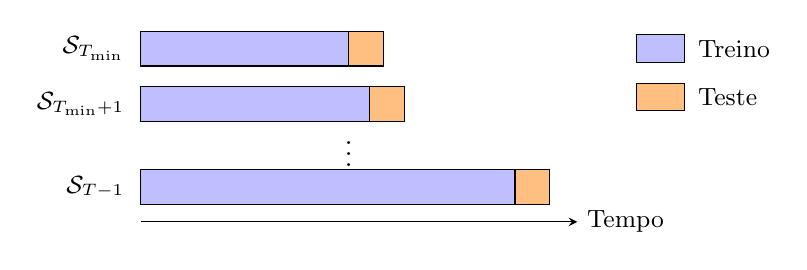
\begin{tikzpicture}[
  block/.style={draw, minimum height=0.45cm, inner sep=0},
  train/.style={block, fill=blue!25},
  test/.style={block,  fill=orange!50},
  scale=0.88
]
\node[left, font=\small] at (-0.1, 2.4) {$\mathcal{S}_{T_{\min}}$};
\node[left, font=\small] at (-0.1, 1.6) {$\mathcal{S}_{T_{\min}+1}$};
\node at (3.0, 1.0) {$\vdots$};
\node[left, font=\small] at (-0.1, 0.4) {$\mathcal{S}_{T-1}$};

\draw[train] (0,    2.15) rectangle (3.0,  2.65);
\draw[test]  (3.0,  2.15) rectangle (3.5,  2.65);

\draw[train] (0,    1.35) rectangle (3.3,  1.85);
\draw[test]  (3.3,  1.35) rectangle (3.8,  1.85);

\draw[train] (0,    0.15) rectangle (5.4,  0.65);
\draw[test]  (5.4,  0.15) rectangle (5.9,  0.65);

\draw[->, >=stealth] (0, -0.1) -- (6.3, -0.1) node[right, font=\small] {Tempo};
\node[draw, fill=blue!25,   minimum width=0.6cm, minimum height=0.35cm] at (7.5, 2.4) {};
\node[right, font=\small] at (7.9, 2.4) {Treino};
\node[draw, fill=orange!50, minimum width=0.6cm, minimum height=0.35cm] at (7.5, 1.7) {};
\node[right, font=\small] at (7.9, 1.7) {Teste};
\end{tikzpicture}
\caption{Protocolo \textit{walk-forward}: a janela de treinamento cresce incrementalmente e o modelo é avaliado apenas em dados futuros, eliminando viés \textit{in-sample}.}
\label{fig:walkforward}
\end{figure}

\subsection{Aplicação Temporal do Protocolo}

Nesta dissertação, o protocolo é parametrizado com $T_{\min} = 12$ ciclos de reposição, resultando em $T - T_{\min} = 26$ pontos de avaliação por série (horizonte total $T = 38$ ciclos). Os modelos de previsão (LSTM, XGBoost, ANN, Croston) são avaliados pelas métricas MASE, sMAPE e RMSSE computadas sobre esses 26 pontos de teste. O mesmo protocolo é aplicado à simulação das políticas de controle de inventário: cada política é executada nos 26 ciclos de avaliação com parâmetros calibrados exclusivamente na janela de treinamento.

A validação \textit{walk-forward} produz estimativas de generalização temporal não viesadas. No processo de seleção contextual, isso é essencial porque as métricas de previsão por série (MASE, sMAPE) alimentam o vetor de entrada do PSE; avaliações apenas \textit{in-sample} tenderiam a inflar artificialmente a acurácia e a distorcer os rótulos de treinamento do meta-modelo.

\subsection{Validação Estatística das Políticas}

O arcabouço inferencial descrito na Seção~\ref{sec:stat_tests} é implementado em quatro etapas:

\begin{enumerate}[(i)]
  \item Wilcoxon pareado: testa se a mediana das diferenças entre a política proposta (GA-DQN / GA-PPO) e cada \textit{baseline} é diferente de zero, para cada KPI e cada quadrante Syntetos-Boylan;
  \item Friedman + Nemenyi: testa simultaneamente se alguma política se distingue das demais e identifica grupos homogêneos via diferença crítica;
  \item Cohen's $d$: quantifica a magnitude prática das diferenças para pares (proposta, \textit{baseline}) em cada KPI;
  \item Análise estratificada: repete os testes por quadrante (Smooth / Erratic / Intermittent / Lumpy) e por estado geográfico, identificando condições sob as quais a arquitetura híbrida é mais vantajosa.
\end{enumerate}

Todos os testes são realizados ao nível de significância $\alpha = 0.05$, com correção para comparações múltiplas quando aplicável. Esse protocolo reduz o risco de interpretações baseadas em diferenças ocasionais entre políticas.

\section{Geração de Rótulos e Treinamento do PSE}
\label{sec:selecao_contextual}

O \textit{Policy Selection Engine} (PSE) transforma os resultados simulados em uma regra de recomendação para séries não vistas. A seleção de políticas é formulada como uma instância supervisionada do problema de seleção de algoritmos (\textit{Algorithm Selection Problem}, ASP): cada série loja-produto é descrita por atributos operacionais, o \textit{benchmark} identifica a política dominante segundo CTI e NS, e o PSE aprende a relação entre perfil operacional e política recomendada.

\subsection{Base Conceitual}

O PSE é uma instância de \textit{meta-aprendizado} aplicado a decisões operacionais: aprende, a partir da experiência acumulada no \textit{benchmark} (``quais políticas funcionaram bem em séries com estas características?''), a mapear o perfil de uma nova série para a política de menor custo total de inventário esperado.

A ideia central é que as características operacionais da demanda: intermitência (ADI), variabilidade (CV$^2$), concentração (\textit{burstiness} $B$), difusividade (entropia $H$), tendência ($\beta_t/\mu$) e sazonalidade ($\rho_S$) capturam estrutura que prediz a dominância de uma família de política sobre as demais. Exemplos de relações esperadas: séries com ADI alto e picos intensos favorecem políticas que toleram longos períodos sem pedido (Jornaleiro, GA-DQN); séries com alta autocorrelação sazonal favorecem políticas que capturam periodicidade (PSO com espaço de busca amplo); séries de baixo volume e alta entropia são estruturalmente não preditíveis e favorecem políticas conservadoras (Jornaleiro).

Sua saída não é apenas um rótulo de algoritmo, mas uma recomendação acionável com probabilidades de confiança, o que permite ao gestor compreender a margem de decisão e selecionar alternativas quando a política recomendada não está disponível.

\paragraph{Fundamentos teóricos.} O PSE fundamenta-se em três pilares convergentes:

\begin{enumerate}[(a)]
  \item Problema de Seleção de Algoritmos, formalizado por \citet{Rice1976AlgorithmSelection}: dado $x$ e um portfólio $\mathcal{A}$, encontrar $a^*(x) = \arg\max_{a \in \mathcal{A}} f(a, x)$. Aqui, $x$ é o vetor $\phi(\mathbf{x}_i)$, $\mathcal{A}$ são as 12 políticas, $a^*(x)$ é a política selecionada para a instância descrita por $x$ e $f$ é o CTI negativo sujeito a NS $\geq \alpha_{\min}$.
  \item Teorema \textit{No Free Lunch}, proposto por \citet{Wolpert1997NoFreeLunch}: ganhos consistentes de desempenho exigem explorar a estrutura específica de cada instância. As características operacionais fornecidas ao AIPE (ADI, CV$^2$, \textit{burstiness}, entropia, sazonalidade) são a estrutura discriminativa que o NFL afirma existir.
  \item Portfólios de algoritmos, discutidos por \citet{Huberman1997AlgorithmPortfolios}: políticas não competem: complementam-se. O PSE explora a diversidade de especializações do portfólio em vez de apostar em um único generalista.
\end{enumerate}

A Figura~\ref{fig:asp_rice} mostra como essa base conceitual é instanciada no AIPE: as séries loja-produto são descritas por características operacionais, as políticas formam o portfólio de alternativas e o desempenho simulado fornece a evidência usada para treinar o seletor contextual.

\begin{figure}[htbp]
\centering
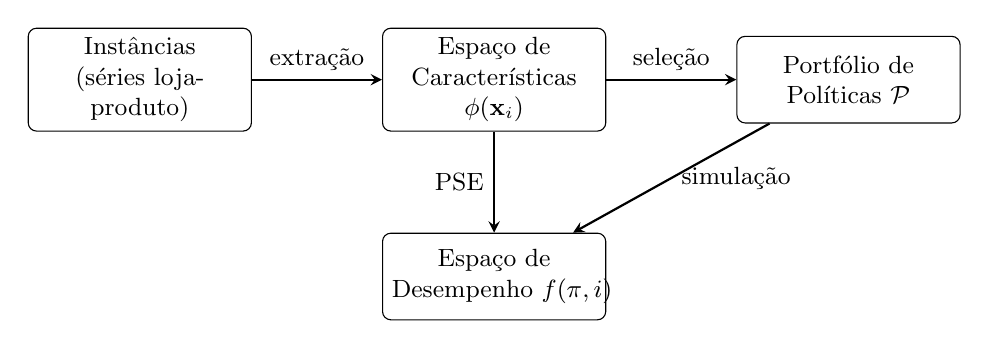
\begin{tikzpicture}[
  box/.style={draw, rounded corners=3pt, minimum width=2.8cm, minimum height=1.1cm,
              text width=2.6cm, align=center, font=\small},
  arr/.style={->, thick, >=stealth}
]
\node[box] (inst) at (0,    0) {Instâncias\\(séries loja-produto)};
\node[box] (feat) at (4.5,  0) {Espaço de\\Características\\$\phi(\mathbf{x}_i)$};
\node[box] (algo) at (9,    0) {Portfólio de\\Políticas~$\mathcal{P}$};
\node[box] (perf) at (4.5, -2.5) {Espaço de\\Desempenho~$f(\pi,i)$};

\draw[arr] (inst) -- node[above, font=\small]{extração} (feat);
\draw[arr] (feat) -- node[above, font=\small]{seleção} (algo);
\draw[arr] (algo) -- node[right, font=\small]{simulação} (perf);
\draw[arr] (feat) -- node[left,  font=\small]{PSE} (perf);
\end{tikzpicture}
\caption{Framework ASP de \citet{Rice1976AlgorithmSelection} instanciado no AIPE: as séries loja-produto constituem as instâncias representadas por características operacionais, as políticas candidatas são avaliadas por simulação e o PSE aprende a recomendar a política viável de menor custo esperado para cada perfil de demanda, respeitando o limiar mínimo de nível de serviço.}
\label{fig:asp_rice}
\end{figure}

\paragraph{Seleção ciente de risco.} Além do critério de menor CTI esperado, o PSE incorpora uma dimensão de risco operacional: a confiança da recomendação (probabilidade máxima do classificador) sinaliza quando o perfil da série está fora da distribuição de treinamento. Recomendações com confiança abaixo de 0.50 são marcadas como incertas, sinalizando ao gestor que nenhuma política apresenta vantagem clara para aquela série específica, padrão que tipicamente indica séries de transição entre quadrantes Syntetos-Boylan.

\subsection{Problema de Seleção}

Dado o vetor de características $\mathbf{x}_i \in \mathbb{R}^{17}$ de uma série $i$ e o conjunto de políticas $\mathcal{P} = \{$EOQ, $(s,S)$, Newsvendor, GA, SA, PSO, DE, DQN, PPO, SARSA, GA-DQN, GA-PPO$\}$, o \textit{Policy Selection Engine} estima:
\begin{equation}
  \hat{\pi}^*(i) = \arg\min_{\pi \in \mathcal{P}} \; \mathbb{E}[\text{CTI}(\pi, i)]
  \quad \text{sujeito a } \mathbb{E}[\text{NS}(\pi, i)] \geq \alpha_{\text{min}},
  \label{eq:policy_selector}
\end{equation}
com $\alpha_{\text{min}} = 0.70$ (configurável). Assim, a política dominante de uma série é a política viável de menor CTI sob NS mínimo; quando nenhuma política atinge NS mínimo, seleciona-se a de maior NS.
Na Equação~\ref{eq:policy_selector}, $\hat{\pi}^*(i)$ é a política recomendada para a série $i$, $\mathcal{P}$ é o portfólio de políticas candidatas, $\text{CTI}(\pi,i)$ é o custo total de inventário da política $\pi$ na série $i$, $\text{NS}(\pi,i)$ é o nível de serviço correspondente e $\mathbb{E}[\cdot]$ indica a média esperada sobre replicações experimentais ou fontes de aleatoriedade do simulador.

\subsection{Rótulos de Política Dominante}

Para cada série loja-produto, o rótulo supervisionado é obtido a partir do \textit{benchmark} simulado das políticas candidatas, seguindo cinco etapas encadeadas: (i) cada política candidata é avaliada no mesmo ambiente de simulação, com as mesmas séries de demanda e os mesmos parâmetros operacionais; (ii) para cada política, são calculadas as métricas CTI, NS, TR, BE e FP ao fim do horizonte de $T$ ciclos; (iii) políticas que não atingem o limiar mínimo de nível de serviço ($\alpha_{\min} = 0{,}70$) são descartadas para fins de rótulo; (iv) entre as políticas restantes, seleciona-se aquela com menor custo total de inventário (CTI), que passa a representar a política dominante da série; (v) o rótulo gerado é atribuído à série e, junto com seu vetor de características operacionais, compõe o \textit{dataset} de treinamento supervisionado do PSE. Esse procedimento transforma a comparação empírica entre políticas em um problema supervisionado de classificação, no qual as características operacionais da série são as entradas e a política dominante é a classe-alvo.

Formalmente, os rótulos $\hat{\pi}^*(i)$ são gerados a partir dos KPIs do \textit{benchmark} (Seção~\ref{sec:benchmark_massivo}): para cada série, agregam-se os KPIs por política (média sobre $n_{\text{rep}} = 5$ replicações) e aplica-se o critério da Equação~\ref{eq:policy_selector}. Isso produz o \textit{dataset} de treinamento $\{(\mathbf{x}_i, \hat{\pi}^*_i)\}_{i=1}^N$, em que $\mathbf{x}_i$ é o vetor de características da série $i$, $\hat{\pi}^*_i$ é seu rótulo de política dominante e $N$ é o número de séries rotuladas.

\subsection{Treinamento do PSE}

Um classificador XGBoost~\citep{ChenGuestrin2016XGBoost} multiclasse é utilizado com hiperparâmetros: $n_{\text{est}}=300$, $\text{depth}=6$, $\eta=0.05$, \textit{subsample} $=0.8$, representando, respectivamente, número de estimadores, profundidade máxima, taxa de aprendizado e fração amostrada de observações por árvore. LightGBM~\citep{Ke2017LightGBM} e RandomForest são alternativas configuráveis.

A avaliação segue validação cruzada estratificada ($k=5$ folds), mantendo a proporção de rótulos por fold. As métricas primárias são:
\begin{itemize}
  \item \textit{Acurácia balanceada} (por conta do desbalanceamento natural de rótulos);
  \item \textit{F1-macro} (trata todas as políticas igualmente);
  \item \textit{F1-weighted} (pondera pelo suporte de cada política).
\end{itemize}

A interpretabilidade do modelo é analisada por importância de características (ganho médio de informação), identificando quais características operacionais são mais discriminativas para a seleção de política. Essa análise permite verificar se o PSE está usando sinais coerentes com a lógica operacional do problema.

\subsection{Saídas do PSE}

O arquivo \texttt{policy\_recommendations.parquet} contém, para cada série: (i) política recomendada; (ii) confiança da previsão; (iii) probabilidades individuais de cada política; (iv) ranking das alternativas candidatas; e (v) justificativa associada ao perfil operacional da série. Isso permite ao gestor entender a margem de decisão e escolher alternativas quando a recomendada não está disponível operacionalmente.

\section{Camada de Aplicação: Recomendações e Reavaliação Periódica}
\label{sec:aplicacao_aipe}

Após o treinamento do PSE, a saída do AIPE é uma recomendação de política de reposição para cada nova série loja-produto descrita por suas características operacionais. Essa recomendação não substitui o sistema transacional da rede varejista, mas fornece uma decisão metodologicamente fundamentada sobre qual política do portfólio deve ser aplicada em cada perfil de demanda.

A aplicação da política gera novos dados de venda, pedidos e estoque, que podem ser incorporados em ciclos posteriores de reavaliação. Nesta dissertação, essa adaptação é tratada como reavaliação periódica: as características da série são recalculadas a cada janela definida, e o PSE pode produzir nova recomendação sem exigir reaprendizado contínuo do meta-modelo.

\section{Artefatos Experimentais e Rastreabilidade}
\label{sec:reporting}

O \textit{pipeline} experimental de apoio ao AIPE produz artefatos com múltiplas funções: (i) figuras comparativas dos cinco KPIs entre as 12 políticas, mostrando heterogeneidade por quadrante Syntetos-Boylan e fronteira de Pareto CTI-NS; (ii) validação estatística visual (\textit{heatmaps} Wilcoxon, Cohen's d, diagrama de diferença crítica); (iii) três \textit{datasets} analíticos: \textit{demand\_features.parquet} (17 características por série), \textit{demand\_profiles.parquet} (classificação POD) e \textit{policy\_recommendations.parquet} (política recomendada pelo PSE com confiança), que alimentam direto a análise da dissertação. Esses artefatos garantem rastreabilidade completa: qualquer leitor pode reconstruir figuras, tabelas e conclusões a partir dos mesmos insumos.

\section{Protocolo Experimental}
\label{sec:protocolo_exp}

Esta seção define o escopo dos experimentos, o número de replicações independentes e o protocolo de validação estatística que garante confiabilidade aos rótulos de treinamento do AIPE. Esses elementos são necessários para que a recomendação aprendida pelo PSE seja baseada em comparações estáveis.

\subsection{Escopo e Replicações}

Esta subseção delimita o escopo experimental adotado para avaliação preliminar do AIPE. Diferentemente da seção de escopo geral apresentada na Introdução, o foco aqui está nas escolhas operacionais do estudo: experimentos avaliados, subconjuntos de dados, políticas comparadas, métricas, replicações e premissas de simulação. Com isso, a seção descreve como a avaliação foi conduzida, sem repetir as delimitações conceituais da pesquisa.

O protocolo experimental distingue dois experimentos avaliados:

\begin{itemize}
  \item Experimento 1, estudo piloto na Paraíba (concluído): 15 lojas $\times$ 1 produto $\times$ 1 estado $\times$ 12 políticas $\times$ 1 replicação (avaliação \textit{in-sample}), produzindo 180 combinações (política, loja).
  \item Experimento 2, expansão na Bahia (concluído): 145 séries do estado da Bahia $\times$ 12 políticas $\times$ 5 replicações com \textit{common random numbers}, habilitando os testes de Wilcoxon e Friedman com poder estatístico adequado.
\end{itemize}

Em ambos os experimentos, as políticas candidatas são avaliadas no mesmo ambiente de simulação e comparadas por custo total de inventário, nível de serviço, ruptura, efeito chicote e frequência de pedidos. As premissas de horizonte temporal, \textit{lead time}, custos, estoque inicial, sementes aleatórias e hiperparâmetros das políticas permanecem fixadas conforme a matriz experimental do Apêndice~\ref{app:reproducibility}, enquanto a ampliação para outros produtos, lojas, estados e regimes de demanda é tratada como etapa futura de expansão nacional.

\subsection{Execução Temporal dos Experimentos}

A avaliação do segundo experimento segue um protocolo de validação temporal em janela deslizante \textit{(rolling horizon)} que integra os insumos experimentais e o núcleo de seleção contextual:

\begin{enumerate}[(i)]
  \item Ingestão de dados: consolidação do histórico $[t-w, t]$ a cada ciclo com atualização das estatísticas locais $\hat{\mu}$ e $\hat{\sigma}$, em que $w$ é o tamanho da janela histórica;
  \item Engenharia de características: recálculo do vetor $\phi(\mathbf{x}_i) \in \mathbb{R}^{17}$ sobre a janela mais recente;
  \item Simulação: execução das 12 políticas candidatas na mesma janela, usando os sinais disponíveis no ciclo de avaliação;
  \item Etiquetagem: aplicação do critério de seleção (Equação~\ref{eq:policy_selector}) para gerar rótulos de treinamento.
\end{enumerate}

\paragraph{Adaptação periódica.} A cada $\Delta t = 6$ ciclos (configurável), o vetor de características é recalculado e o POD é reavaliado. Se a série migrar entre quadrantes Syntetos-Boylan, o PSE emite nova recomendação de política para o próximo ciclo operacional. Esse mecanismo não exige reaprendizado do meta-modelo, apenas recálculo das características e consulta ao classificador: (a) recalcular $\phi(\mathbf{x}_i)$; (b) reclassificar POD; (c) consultar PSE: $\hat{\pi}^*(i) \leftarrow f(\phi(\mathbf{x}_i))$; (d) aplicar. Essa reatividade é a distinção central do AIPE: a relação regime$\rightarrow$política não é regra manual estática, mas modelo aprendido que se adapta conforme o padrão operacional evolui.

\subsection{Síntese do Protocolo}

O \textit{pipeline} experimental é implementado com rastreabilidade completa de insumos, configurações e artefatos. Reprodutibilidade é garantida por: versionamento Git de código e parâmetros, sementes aleatórias fixas por experimento, hashes de \textit{datasets} de entrada, e documentação de dependências de software. Todos os dados, scripts e resultados são versionados e criptograficamente auditáveis, permitindo reconstruir integralmente todos os experimentos a partir dos mesmos parâmetros. A matriz completa dos parâmetros experimentais, configurações e artefatos necessários à reprodução das políticas avaliadas é apresentada no Apêndice~\ref{app:reproducibility}.

A Tabela~\ref{tab:met_comp_proposta} resume o papel relativo das principais famílias de métodos no contexto MEIO, destacando que a escolha metodológica envolve compromisso entre escalabilidade, interpretabilidade, custo computacional e forma de tratamento das restrições.

\begin{table}[htbp]
\centering
\small
\caption{Comparação entre famílias de métodos no contexto MEIO.}
\label{tab:met_comp_proposta}
\begin{tabular}{lcccc}
\toprule
Método & Escalabilidade & Interpretabilidade & Custo comput. & Restrições \\
\midrule
MILP/ILP & Baixa & Alta & Alto & Exato \\
Meta-heurísticas (GA/SA/PSO/DE) & Alta & Média & Médio & Penalização \\
RL isolado (DQN/PPO/SARSA) & Média & Baixa & Alto & Indireto \\
Híbrido GA-RL & Alta & Média & Médio & Penalização \\
\bottomrule
\end{tabular}
\end{table}
